\chapter{Ergebnisse} \label{sec:results}

Nachfolgend ist eine Beispielabbildung und eine Beispieltabelle zu sehen.
Die Abbildung ist als \textit{svg}-Datei abgelegt und wird mit Inkscape automatisch in eine \textit{pdf}-Datei umgewandelt.

\begin{figure}
	\centering
	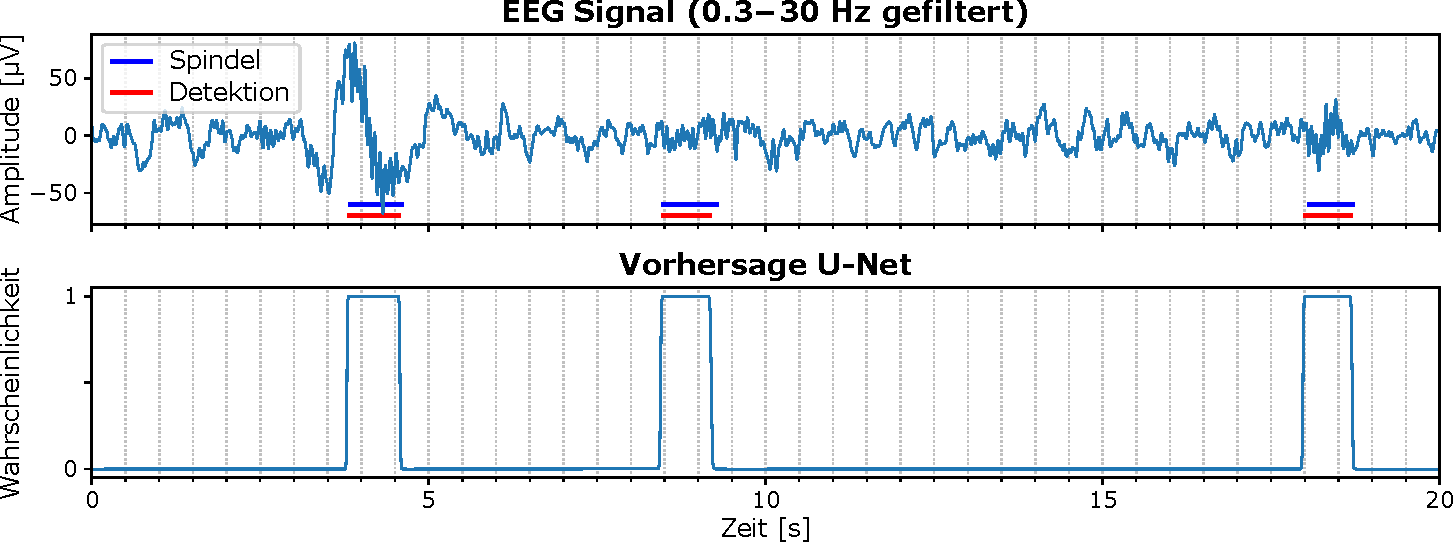
\includegraphics[width=\linewidth]{images/spindle-detection-u-net_svg-raw}
	\caption{
		Detektion des U"~Net Modells beispielhaft auf \SI{20}{\s} der Testdaten.
		In der ersten Zeile ist das Breitband"=Signal mit den annotierten und detektierten Spindeln und in der zweiten Zeile die vom Modell ausgegebene Wahrscheinlichkeit für eine Schlafspindel abgebildet.
	}
	\label{fig:results:spindle-detection-u-net}
\end{figure}

\begin{table}
	\centering
	\begin{threeparttable}
		% Tabellen ohne Nutzung von \rowstyle können ohne ^ und + angelegt werden
		\begin{tabular}{@{}^l+c+c+c+c+c+c+c+c+c@{}}
			\toprule
			& \multicolumn{3}{c}{beide Kohorten} & \multicolumn{3}{c}{jüngere Kohorte} & \multicolumn{3}{c}{ältere Kohorte} \\
			\cmidrule(l){2-4} \cmidrule(l){5-7} \cmidrule(l){8-10}
			Detektor & Recall & Prec & F1 & Recall & Prec & F1 & Recall & Prec & F1 \\
			\midrule
			Experte\tnote{1,2} & \num{0.72} & \num{0.78} & \num{0.72} & \num{0.76} & \num{0.81} & \num{0.76} & \num{0.66} & \num{0.74} & \num{0.65} \\
			A7 \autocite{Lacourse2019}\tnote{1} & \num{0.73} & \num{0.71} & \num{0.72} & \num{0.75} & \num{0.73} & \num{0.74} & \num{0.70} & \num{0.69} & \num{0.70} \\
			A7 \autocite{Lacourse2019}\tnote{3} & \num{0.76} & \num{0.70} & \num{0.73} & \num{0.78} & \num{0.70} & \num{0.74} & \num{0.73} & \num{0.69} & \num{0.71} \\
			\rowstyle{\color{red}}
			U-Net & \num{0.79} & \num{0.85} & \num{0.82} & \num{0.82} & \num{0.85} & \num{0.84} & \num{0.73} & \num{0.85} & \num{0.79} \\
			\bottomrule
		\end{tabular}
		\begin{tablenotes}
			\item[1]{Wie in \autocite{Lacourse2020} berichtet.}
			\item[2]{Durchschnittlicher Wert der Experten bezogen auf den Gruppenkonsens ohne den jeweiligen Experten.}
			\item[3]{Auf den hier genutzten Testdaten ausgewertet.}
		\end{tablenotes}
	\end{threeparttable}
	\caption{
		Ergebnisse auf den Testdaten bei der Evaluierung beider Kohorten und bei der Evaluierung jeweils einer Kohorte.
		Die Ergebnisse aus \autocite{Lacourse2020} sind auf allen $n=180$ Patienten berechnet worden, die hier verwendeten Testdaten umfassen $n=36$ Patienten.
		Angegeben sind jeweils Recall, Precision (\textit{Prec}) und F1 Score bei \SI{20}{\percent} Overlap Threshold.
	}
	\label{tab:results:f1-scores}
\end{table}

